\section{Architektur}

\subsection{Maschinentyp}

\begin{frame}[fragile]{\insertsubsection}
 \begin{itemize}
  \item UMach ist eine registerbasierte RISC Maschine.
        
        Wenige Befehle (69) mit fester Länge.        
  \item Load/Store Speicherzugriff über Registerangabe.
\begin{lstlisting}
LW   R1 R2 # R1 $\gets$ mem(R2)
SW   R1 R2 # R1 $\to$ mem(R2)
\end{lstlisting}
  \item Big endian
  \item Port I/O
\begin{lstlisting}
IN  R17 R18 R19
OUT R1  R2  R3
\end{lstlisting}
 \end{itemize}
\end{frame}


\subsection{Register}

\begin{frame}{\insertsubsection}
 \begin{itemize}
   \item 32 Allzweckregister und 13 Spezialregister.
   \item Jedes Register ist genau 32 Bit lang.
   \item Register werden intern durch Nummern identifiziert:
         Register Nummer 0, 1, 2\ldots{} 44.
 \end{itemize}
\end{frame}


\subsubsection{Allzweckregister}

\begin{frame}{\insertsubsubsection}
 \begin{itemize}
   \item Register mit Nummern 1 bis 32 können frei verwendet werden.
   \item Werden von der Maschine ohne explizite Anweisung nicht geändert, außer
         dass sie mit Null initialisiert werden.
   \item Namen entsprechen der Nummerierung:\\
         $R1$, $R2$, \ldots{} $R32$.
 \end{itemize}
\end{frame}



\subsubsection{Spezialregister}

\begin{frame}{\insertsubsubsection}
 \begin{itemize}
   \item Dienen der Steuerung der Maschine.
   \item Haben besondere Aufgaben.
   \item Werden von der Maschine im Betrieb verändert.
   \item Meisten sind schreibgeschützt.
 \end{itemize}
\end{frame}



\begin{frame}{\insertsubsubsection{} - Liste}
 \begin{tabular}{lcl}
Name  & Nummer & Beschreibung                \\\toprule
PC    & 33     & Program Counter             \\ 
DS    & 34     & Data Section (begin)        \\ 
HS    & 35     & Heap Section (first byte)   \\ 
HE    & 36     & Heap Section (last byte)    \\ 
SP    & 37     & Stack Pointer               \\
FP    & 38     & Frame Pointer               \\
IR    & 39     & Instruction Register        \\
STAT  & 40     & Status Register             \\
ERR   & 41     & Error Register              \\
HI    & 42     & Higher 32 Bits (Division, Multiplik.) \\
LO    & 43     & Lower 32 Bits (Division, Multiplik.)  \\
CMPR  & 44     & Ergebniss von CMP           \\
ZERO  & 0      & Immer konstant Null         \\\bottomrule
 \end{tabular}
\end{frame}



\subsection{Befehlsformat}

\begin{frame}{\insertsubsection}
\framesubtitle{Allgemeines Format}
 \begin{center}
   
\begin{tikzpicture}

\tikzstyle{lab}=[midway,yshift=-10pt,align=center,anchor=north]

  \matrix (m) 
 [matrix of nodes,
  nodes={draw,text height=2ex,text depth=0.25ex,
  minimum width=5em,font=\ttfamily}]
 {
    0x30 & 0x03 & 0x01 & 0x02 \\
 };
 
 \draw[decorate] (m-1-1.south west) -- (m-1-1.south east) 
  node [lab] {Befehl};
 \draw[decorate] (m-1-2.south west) -- (m-1-4.south east) 
  node [lab] {Argumente};
\end{tikzpicture}

 \end{center} 
\end{frame}


\begin{frame}{\insertsubsection}
 \begin{center}
  \begin{tabular}{l||c|c|c}
    \toprule
    Format & zweites Byte  & drittes Byte  & viertes Byte \\\toprule
    000 & \multicolumn{3}{c}{nicht verwendet}           \\\midrule
    NNN & \multicolumn{3}{c}{3 Bytes Zahl}              \\\midrule
    R00 & $R_{1}$ & \multicolumn{2}{c}{nicht verwendet} \\\midrule
    RNN & $R_{1}$ & \multicolumn{2}{c}{2 Bytes Zahl}    \\\midrule
    RR0 & $R_{1}$ & $R_{2}$ &  nicht verwendet          \\\midrule
    RRN & $R_{1}$ & $R_{2}$ &  1 Byte Zahl              \\\midrule
    RRR & $R_{1}$ & $R_{2}$ & $R_{3}$                   \\\bottomrule
  \end{tabular}
\end{center}
($R_{1}$, $R_{2}$, $R_{3}$: erste, zweite, dritte Registernummer)

Alle Zahlenangaben: big endian.
\end{frame}



\begin{frame}{\insertsubsection{} - Beispiel RRR}
 \texttt{ADD}: drei Registernummern.
 \begin{center}
   
\begin{tikzpicture} [font=\ttfamily]

\tikzstyle{lab}=[midway,yshift=-10pt,align=center,anchor=north]

  \matrix (m) 
 [matrix of nodes,
  nodes={draw,text height=2ex,text depth=0.25ex,
  minimum width=5em}]
 {
    0x30 & 0x03 & 0x01 & 0x02 \\
 };
 
 \draw[decorate] (m-1-1.south west) -- (m-1-1.south east) node [lab] {ADD};
 \draw[decorate] (m-1-2.south west) -- (m-1-2.south east) node [lab] {R3};
 \draw[decorate] (m-1-3.south west) -- (m-1-3.south east) node [lab] {R1};
 \draw[decorate] (m-1-4.south west) -- (m-1-4.south east) node [lab] {R2};
\end{tikzpicture}

 \end{center}
\end{frame}

\begin{frame}{\insertsubsection{} - Beispiel RNN}
 \texttt{DIVI}: eine Registernummer und eine 2-Byte Zahl.
 \begin{center}
   
\begin{tikzpicture} [font=\ttfamily]

\tikzstyle{lab}=[midway,yshift=-10pt,align=center,anchor=north]

  \matrix (m) 
 [matrix of nodes,
  nodes={draw,text height=2ex,text depth=0.25ex,
  minimum width=5em}]
 {
    0x3D & 0x03 & 0x01 & 0x02 \\
 };
 
 \draw[decorate] (m-1-1.south west) -- (m-1-1.south east) node [lab] {DIVI};
 \draw[decorate] (m-1-2.south west) -- (m-1-2.south east) node [lab] {R3};
 \draw[decorate] (m-1-3.south west) -- (m-1-4.south east) node [lab] {0x0102};
\end{tikzpicture}

 \end{center}
\end{frame}

\begin{frame}{\insertsubsection{} - Beispiel NNN}
 \texttt{JMP}: ein 3-Byte Offset (vorzeichenbehaftet).
 \begin{center}
   
\begin{tikzpicture} [font=\ttfamily]

\tikzstyle{lab}=[midway,yshift=-10pt,align=center,anchor=north]

  \matrix (m) 
 [matrix of nodes,
  nodes={draw,text height=2ex,text depth=0.25ex,
  minimum width=5em}]
 {
    0x88 & 0xFF & 0xFF & 0xFD \\
 };
 
 \draw[decorate] (m-1-1.south west) -- (m-1-1.south east) node [lab] {JMP};
 \draw[decorate] (m-1-2.south west) -- (m-1-4.south east) node [lab] {-3};
\end{tikzpicture}

 \end{center}
\end{frame}

\subsection{Befehlsmenge}

\begin{frame}{\insertsubsection}
\begin{enumerate}
  \item Kontrollinstruktionen: \texttt{NOP}, \texttt{EOP}
  \item Lade- und Speicherbefehle: 
        \texttt{SET}, \texttt{LW}, \texttt{SB}, \texttt{PUSH}
  \item Arithmetische Instruktionen:
        \texttt{ADD}, \texttt{SUB}, \texttt{INC}
  \item Logische Instruktionen:
        \texttt{AND}, \texttt{XOR}, \texttt{SHL}, \texttt{ROTL}
  \item Vergleichsinstruktionen:
        \texttt{CMP}, \texttt{CMPI}
  \item Sprunginstruktionen:
        \texttt{JMP}, \texttt{BE}, \texttt{BL}
  \item Unterprogramminstruktionen:
        \texttt{CALL}, \texttt{RET}, \texttt{GO}
  \item Systeminstruktionen:
        \texttt{INT}
  \item I/O Instruktionen:
        \texttt{IN}, \texttt{OUT}
\end{enumerate}
Insgesamt 69 Befehle.
\end{frame}



\subsection{Speichermodell}

\begin{frame}{\insertsubsection}
 \framesubtitle{Speichersegmente}
 \begin{center}
   
\begin{tikzpicture}
\tikzset{
  mmatrix/.style={
    matrix of nodes,
    nodes={
      draw,
      minimum height=8ex,
      text depth=0ex,
      align=center,
      anchor=center,
      font=\small
    }
  }
};

\tikzstyle{lab}=[yshift=-2ex,anchor=center]

 \matrix (m) [mmatrix]
 {
    |[text width=1.7cm]|Interrupt\-tabelle & 
    Programm & Daten & Heap & frei & Stack \\
 };

  \draw[thick] (m-1-1.north west) -- ++(0,-2) node[lab] {0};
  \draw[thick] (m-1-1.north east) -- ++(0,-2) node[lab] {256};
  \draw[thick] (m-1-2.north east) -- ++(0,-2) node[lab] {DS};
  \draw[thick] (m-1-3.north east) -- ++(0,-2) node[lab] {HS};
  \draw[thick,dashed] (m-1-4.north east) -- ++(0,-2) node[lab] {HE};
  \draw[thick,dashed] (m-1-5.north east) -- ++(0,-2) node[lab] {SP};
  \draw[thick] (m-1-6.north east) -- ++(0,-2) node[lab] {max};
\end{tikzpicture}

 \end{center}
 Segmentation Fault: schreiben in Code-Segment.
 
 Stack Overflow: Befehl \texttt{PUSH} führt zum Überlappen der Register
\texttt{SP} und \texttt{HE}.
\end{frame}


\begin{frame}[fragile]{Heap und Stack Manipulieren}
 \begin{lstlisting}
  ADDI HE HE 128
  # ...
  SUBI HE HE 128
 \end{lstlisting}
 Speicher auf dem Heap reservieren erfolgt dadurch, dass der Inhalt des
 Registers \texttt{HE} (Heap End) hochgezählt wird. Speicher freigeben durch
 runterzählen.
 
 \begin{lstlisting}
  SUBI SP SP 32
  # ...
  ADDI SP SP 32
 \end{lstlisting}
 Lokaler Speicher wird durch Veränderung des Registers \texttt{SP} (Stack
 Pointer) erreicht.
\end{frame}



\subsection{I/O}

\begin{frame}{Port I/O}
   \begin{center}
  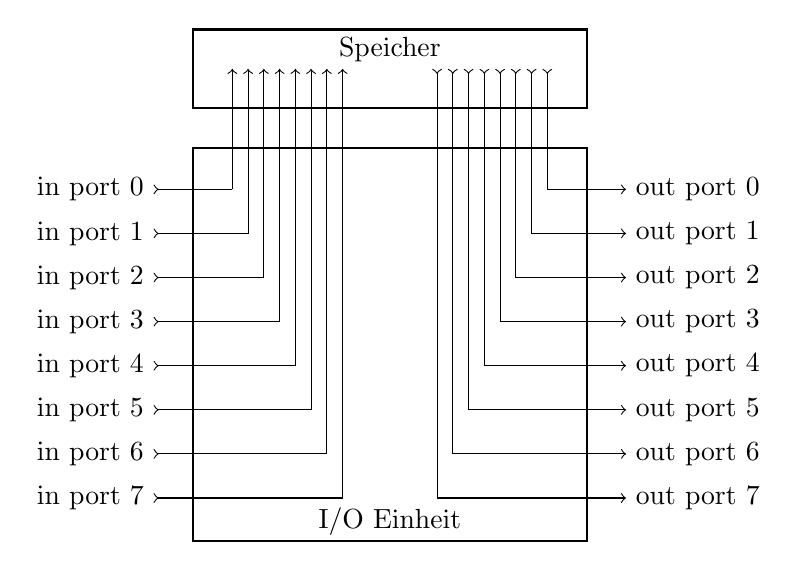
\begin{tikzpicture}  
  \draw[thick] (0,0) rectangle (5,5);
  \node at     (2.5,0.25) {I/O Einheit};
  
  \foreach \y [count=\i from 0, evaluate=\i as \p using int(7-\i),
                                evaluate=\i as \s using (0.5 + \p/5),
                                evaluate=\i as \q using (4.5 - \p/5)]
  in {0.55, 1.11, ...,5}
  {
      \draw[->] (4.5, \y) -- ++(+1,0) node [right] {out port \p};
      \draw[-<] (0.5, \y) -- ++(-1,0) node [left]  {in port  \p};
      \draw[->] (0.5, \y) -| (\s,6);
      \draw[>-] (\q,6)    |- (4.5,\y);
  }
  
  \draw[thick] (0,5.5) rectangle (5,6.5);
  \node at     (2.5, 6.25) {Speicher};

\end{tikzpicture}
 

 \end{center}
\end{frame}


\begin{frame}{Datentransfer}
 \begin{itemize}
   \item Direkt zwischen Speicher und I/O-Ports.
   \item Blockiert die Maschine solange der Transfer noch nicht fertig ist.
 \end{itemize}
\end{frame}


\begin{frame}{Ausgabe}
 Die Ausgabe erfolgt durch verwendung des Befehls \texttt{OUT}
 \begin{center}
   
\begin{tikzpicture}

\tikzstyle{lab}=[midway,yshift=-10pt,align=center,anchor=north,font=\small]

  \matrix (m) 
 [matrix of nodes,
  nodes={draw,
         text height=2ex,text depth=0.25ex,
         minimum width=5em,
         font=\ttfamily}]
 {
    OUT & R1 & R2 & ZERO \\
 };
 
 \draw[decorate] (m-1-1.south west) -- (m-1-1.south east) node [lab] {Ausgabe};
 \draw[decorate] (m-1-2.south west) -- (m-1-2.south east) 
                 node [lab] {Adresse\\ im Speicher};
 \draw[decorate] (m-1-3.south west) -- (m-1-3.south east) 
                 node [lab] {Anzahl\\ bytes};
 \draw[decorate] (m-1-4.south west) -- (m-1-4.south east) 
                 node [lab] {Portnummer};
 
\end{tikzpicture}

 \end{center}
\end{frame}


\begin{frame}{Eingabe}
 Die Eingabe erfolgt durch verwendung des Befehls \texttt{IN}
 \begin{center}
  \input{./Arch/io1}
 \end{center}
\end{frame}


\subsection{Interrupts}

\begin{frame}{\insertsubsection}
 Unterbrechungen im normalen Programmfluss.
 \begin{itemize}
   \item Mit einer Interruptnummer versehen (\texttt{INT 26}).
   \item Können abgefangen werden (interrupt handlers).
   \item Analog zu \glqq exceptions\grqq{} in Java/C++.
 \end{itemize}
\end{frame}



\begin{frame}{Arten von Interrupts}
 \begin{enumerate}
  \item Hardware-Interrupts: wenn etwas schief mit einem Befehl geht:
        Division durch Null, Stack Overflow, falsche Befehlsnummer, ungültige
        Speicheraddresse, schreiben in das Codesegment, etc.
  \item Software-Interrupts: werden vom Programmierer durch den Befehl 
        \texttt{INT} angestoßen.
 \end{enumerate}
\end{frame}


\begin{frame}{Interrupttabelle}
 \begin{itemize}
   \item Startet an der Addresse Null.
   \item 64 Einträge, jeweils 32 Bit groß.
   \item Jeder Eintrag entspricht einer Interruptnummer.\\
         Interrupt 26 $\to$ Adresse $26 \cdot 4 = 104$.
   \item Eintrag enthält entweder Null oder die Adresse eines
         \glqq interrupt handlers\grqq.
 \end{itemize}
\end{frame}



\begin{frame}{Wie läuft ein Interrupt ab}
 \begin{center}
  \begin{tikzpicture} [->,node distance=1.8cm,auto]

\tikzset{every label/.style={font=\scriptsize,red!80!black}}
\tikzstyle{start}=[draw=blue!20!black,circle]
\tikzstyle{block}=[draw]
\tikzstyle{end}  =[draw=green!60!black,rounded corners,double]
\tikzstyle{err}  =[draw=red!60!black,rounded corners,double]
\tikzstyle{ask}  =[draw,diamond,align=center,text badly centered,inner sep=0pt,
                   text width=4em,aspect=2]
\tikzstyle{away} =[node distance=4cm]

 
 
 \node[start,label=below:{segfault}]
                              (A) {\texttt{INT} $x$};
 \node[ask,right of=A,away]   (B) {$x \geq 0 \;\land\; x \leq 63$?};
 \node[block,right of=B,away] (C) {$x \gets 0$};
 \node[block,below of=B]      (D) {$y \gets$ interrupt\_table[$x$]};
 \node[ask,below of=D]        (E) {$y = 0$?};
 \node[err,right of=E,away]   (F) {stop Umach};
 \node[end,below of=E]        (G) {\texttt{PUSH PC}; \texttt{GOTO} $y$};

 \draw (A) --                  (B);
 \draw (B) -- node {nein}      (C);
 \draw (B) -- node {ja}        (D);
 \draw[rounded corners] (C) |- (D);
 \draw (D) --                  (E);
 \draw (E) -- node {ja}        (F);
 \draw (E) -- node {nein}      (G);
\end{tikzpicture}




 \end{center}
\end{frame}



\section{Implementierung}

\subsection{Programmablauf}

\begin{frame}[fragile]{\insertsubsection}
 Die Maschine führt grundsätzlich zwei Schritte aus, die sich immer wieder
 wiederholen: fetch und execute. 
 \begin{lstlisting}
void core_run_program(void)
{
    while (running) {
        core_fetch();
        core_execute();
    }
}
 \end{lstlisting}
\end{frame}


\begin{frame}[fragile]{Fetch}
 Fetch: die nächste Instruktion aus dem Speicher holen.
\begin{lstlisting}
void core_fetch(void)
{
    if (! running) { return; }
    mem_read               // read from mem
    ( instruction,         // whereto
      registers[PC].value, // wherefrom
      4                    // how much
    );
}
\end{lstlisting}
Lese 4 Bytes aus dem Speicher ab der Adresse \texttt{\$PC} in den globalen
Puffer \texttt{uint8\_t instruction[4]}.
\end{frame}



\begin{frame}[fragile]{Execute}
 Befehl ausführen und \texttt{PC} inkrementieren.
\begin{lstlisting}
struct command *cmd = 
       command_by_opcode(instruction[0]);
if   (cmd != NULL) 
     { cmd->opfunc();              } 
else { interrupt(INT_INVALID_CMD); }
registers[PC].value += 4;
\end{lstlisting}

Es wird nach einem Funktionszeiger gesucht, der dem Befehlscode entspricht.
Fall vorhanden, ausführen. Falls nicht, Interrupt generieren.
\end{frame}


\subsection{Sprungtabellen}

\begin{frame}{Frage}
  Wie wird schnell nach einem Funktionszeiger gesucht?
\end{frame}


\begin{frame}[fragile]{\insertsubsection{} -- Auszug}
\begin{lstlisting}
struct command opmap[OPMAX] = {
/*  opcode ->  function
    ----------------------*/
    [0x00]  =  core_nop,
    [0x04]  =  core_eop,
    [0x10]  =  core_set,
    ....
    [0x90]  =  core_go ,
    [0x91]  =  core_cal,
    [0x92]  =  core_ret,
    [0xA0]  =  core_int,
    [0xB0]  =  core_in ,
    [0xB8]  =  core_out,
};
\end{lstlisting}
Suchaufwand $O(1)$. Schneller geht's nicht.
\end{frame}

\begin{frame}[fragile]{Suchen in der Sprungtabelle}
 Wie findet mal die Funktion, die einem Befehlscode entspricht?
\begin{lstlisting}
struct command* command_by_opcode
(int opcode)
{
    return opmap[opcode];
}
\end{lstlisting}
(Vereinfachte Version)
\end{frame}


\begin{frame}[fragile]{Ein Beispiel: \texttt{ADD}-Befehl}
\begin{center}
   
\begin{tikzpicture} [font=\ttfamily]

\tikzstyle{lab}=[midway,yshift=-10pt,align=center,anchor=north]

  \matrix (m) 
 [matrix of nodes,
  nodes={draw,text height=2ex,text depth=0.25ex,
  minimum width=5em}]
 {
    0x30 & 0x03 & 0x01 & 0x02 \\
 };
 
 \draw[decorate] (m-1-1.south west) -- (m-1-1.south east) node [lab] {ADD};
 \draw[decorate] (m-1-2.south west) -- (m-1-2.south east) node [lab] {R3};
 \draw[decorate] (m-1-3.south west) -- (m-1-3.south east) node [lab] {R1};
 \draw[decorate] (m-1-4.south west) -- (m-1-4.south east) node [lab] {R2};
\end{tikzpicture}

 \end{center}
 
Eintrag in der Sprungtabelle:
\begin{lstlisting}
[0x30] = core_add,
\end{lstlisting}
\end{frame}


\begin{frame}[fragile]{\texttt{ADD} -- Implementierung}
\begin{lstlisting}
int core_add(void) {
    int32_t a = 0; 
    int32_t b = 0;

    read_register  (instruction[2], &a   );
    read_register  (instruction[3], &b   );
    write_register (instruction[1], a + b);       
    return 0;
}
\end{lstlisting}
(Veränderte Version, Error Checks gelöscht).
\end{frame}



